\documentclass[a4,12pt]{article}

\usepackage[utf8]{inputenc}
\usepackage[spanish]{babel}
\usepackage[margin=1.5cm]{geometry}
\usepackage{graphicx}
\usepackage{color}
\usepackage{import}



\usepackage{hyperref}

\parindent 0em

%\usepackage{times}
\renewcommand{\familydefault}{\sfdefault}

\title{Breve introducción a GNU OCTAVE}
\author{Youssef Said Khloufi}
%\date{}

\begin{document}

\maketitle

\begin{abstract}
Este documento explica de manera muy breve los fundamentos y características principales del software libre GNU Octave.

\end{abstract}

\tableofcontents
\newpage

\section{Introducción}

OCTAVE : Lenguaje numérico de programación de libre acceso.

\subsection{Características principales del OCTAVE}

- Programa específico de Cálculo Numérico.\\
• Sólo opera con Números.\\
• Se puede considerar como una calculadora programable muy potente.\\
\medskip\\
-Programa muy popular entre estudiantes, ingenieros, técnicos e investigadores debido a sus características:\\
• Programa de libre acceso.\\
• Programa interactivo.\\
• Capacidades Gráficas sencillas.\\
• Posee gran cantidad de Funciones de todos los tipos.\\
• Lenguaje de programación de alto nivel similar a Fortran, C, Pascal o Basic, pero más  fácil de aprender.\\
Su lenguaje de programación es igual al de MATLAB.\\

\subsection{Acceso al OCTAVE desde el entorno Unix}

• Ejecutar la instrucción octave desde cualquier ventana\\
• Aparece la siguiente ventana del octave:\\
\begin{verbatim}
    octave:1>
\end{verbatim}

\subsection{Accesos al OCTAVE desde windows}

• Hacer doble click sobre el icono de OCTAVE.\\
• Al igual que en el entorno Unix , aparece la ventana del octave (consola).\\

\subsection{Algunas instrucciones de utilidad }

-pwd: nos dice en que directorio nos encontramos.\\
-ls: nos da una lista de los ficheros y los directorios\\
-cd: nombre nos permite cambiar al directorio nombre.\\

\subsection{Operaciones básicas.}

\begin{verbatim}
    + adición
    - sustracción
    * multiplicación
    ^ potenciación
    \ división izquierda
    / división derecha
\end{verbatim}

\begin{verbatim}
    exp   log   exponencial y logaritmo neperiano
    sin   cos   seno y coseno
    abs   sqrt  valor absoluto y raíz cuadrada
    round floor ceil funciones que redondean
\end{verbatim}

Ejemplos:

\begin{verbatim}
    > 2 + 3         > 2 * 2
    ans = 5          ans = 4

    > sin(pi/6)     > 2/6
    ans = 0.50000    ans =0.33333

    > log(5^3)      > round(4.5)
    ans = 4.8283     ans = 5

    > ceil(4.5)     > floor(4.5)
    ans = 5          ans = 4
\end{verbatim}

• Observe que: los () se reservan sólo para escribir el argumento de las funciones.\\

\subsection{Ayudas y normas generales del OCTAVE}

• El comando help nos proporciona información sobre las funciones del OCTAVE:\\
\begin{verbatim}
    > help round   % redondea al entero mas cercano
    > help floor   % redondea por defecto
    > help ceil    % redondea por exceso
\end{verbatim}
• Las flechas: arriba y abajo permiten recuperar comandos anteriores.\\
• Las flechas: izquierda y derecha permiten movernos a lo largo de una línea de instrucciones y corregirla.\\
• OCTAVE distingue entre mayúsculas y minúsculas:\\
\begin{verbatim}
    > ceil(2.3)
    ans = 3
\end{verbatim}
NO es lo mismo que:\\
\begin{verbatim}
    > Ceil(2.3)
    error: ‘Ceil’ undefined near line 22 column 1
\end{verbatim}
• Podemos asignar variables con determinados nombres a las expresiones numéricas (números,constantes).\\
\begin{verbatim}
    > m = 9.11e-31; q = -1.6e-19;
    > r = abs(q)/m
    r = 1.7563e+11
    > 3e+8
    ans = 300000000
    > m*(ans^2)
    ans = 8.1990e-014
\end{verbatim}
• Los nombres de estas variables pueden formarse utilizando letras,dígitos, etc.\\
• Las variables se pueden borrar con el comando clear nombre.\\
• Asignación por defecto: si a una expresión numérica no le asignamos un nombre, OCTAVE crea la variable ans.\\
• El comando who nos permite conocer los nombres de las variables asignadas. Ejecute who\\

\section{Vectores}

vacio.

\subsection{Vectores fila y vectores columnas}

\subsection{Utilización de los dos puntos}

\subsection{Funciones sobre los vectores}

\subsection{Operaciones vectoriales y Operaciones puntuales}

\section{Editor del OCTAVE. Programación}

\subsection{Tipos de m-files}

\section{Gráficos}

\subsection{Gráficos en 2 dimensiones}

problema
\begin{figure}
  \centering
    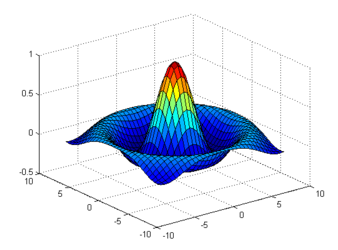
\includegraphics{graficos/octave}
\end{figure}

\section{Grabar y leer datos en ficheros. Impresión de las gráficas}

\end{document}
